\section{Auswertung}
\label{sec:Auswertung}

Die Literaturwerte für die Schallgeschwindigkeiten
\begin{align}
  c_\text{Acryl} & = \SI{2730}{\meter\per\second} \\
  c_\text{Wasser} & = \SI{1480}{\meter\per\second}
\end{align}
werden der Quelle \cite{schall} entnommen.

\subsection{Längenmessungen am Acrylblock zur Überprüfung}

Für die Größenabmessungen am Acrylblock werden folgende Werte aufgenommen:
\begin{align}
  t/\si{\centi\meter}: & (4.000 , 4.000) \\
  b/\si{\centi\meter}: & (15.025 , 15.000) \\
  h/\si{\centi\meter}: & (8.040, 8.040)
\end{align}
Daraus folgen die gemittelten Werte für Tiefe, Breite und Höhe
\begin{align}
  \bar{t} & = \SI{4.00}{\centi\meter} \\
  \bar{b} & = \SI{15.01(2)}{\centi\meter} \\
  \bar{h} & = \SI{8.04}{\centi\meter}.
  \label{eqn:AbmessungenAcryl}
\end{align}
Um Vergleichswerte für die mit den Scans aufgenommenen Messwerte zu haben,
werden weitere Abmessungen mit einer Schieblehre gemessen.
Die Position der Löcher werden bestimmt, indem der Abstand zwischen der
unteren Kante des Acrylblocks zur Mitte des jeweiligen Lochs gemessen wird.
Die aufgenommenen Längen dafür, sowie für die Größe der Löcher sind in
Tabelle \ref{tab:AbmessungenAcryl} abgebildet.

\subsection{Untersuchung des Acrylblocks mit dem A-Scan}

Die gemessenen Laufzeiten der Schallwellen am Acrylblock bis zu den jeweiligen
Störstellen und zurück zum Sender sind in Tabelle \ref{tab:AScanZeiten} dargestellt.
Der Wert für $a_8$ in der zweiten Messung kann mit dem AScan nicht festgestellt
werden und daher auch nicht die zugehörige Breite der Störstelle.
Nachdem die Laufzeitkorrektur
\begin{align}
  t_\text{l,A} = \SI{0.5}{\micro\second}
\end{align}
von den Werten abgezogen wird, wird mit der Formel \eqref{eqn:SchallStrecke}
jeweils die Strecke zu jeder Störstelle bestimmt.
Die berechneten Werte sind in Tabelle \ref{tab:AScanStrecken}
abgebildet.
Aus diesen Daten wird die Dicke der einzelnen Störstellen jeweils mit
\begin{align}
  d_\text{A} & = h - s_\text{A,1} - s_\text{A,2}
  \label{eqn:Dicke}
\end{align}
bestimmt. Die Ergebnisse sind in Tabelle \ref{tab:AScanDicken} aufgelistet.

\subsection{Untersuchung des Acrylblocks mit dem B-Scan}

Die Ergebnisse der Untersuchungen mit dem B-Scan sind in den Abbildungen
\ref{fig:BScan1} und \ref{fig:BScan2} dargestellt.
Daraus werden jeweils die Laufzeiten, abzüglich der Laufzeitkorrektur
\begin{align}
  t_\text{l,B} = \SI{3}{\micro\second},
\end{align}
und damit mit der Formel
\ref{eqn:SchallStrecke} die Strecken zu den
jeweiligen Störstellen bestimmt. Der Durchmesser wird dann wie beim A-Scan mit
\eqref{eqn:Dicke} ausgerechnet
Die Werte dafür sind in Tabelle \ref{tab:BScanZeitenStreckenDicken}
dargestellt. Bei dem zweiten Scan kann erneut kein Messwert für die Laufzeit
zu $a_8$ aufgenommen werden und daher auch kein Durchmesser für diese
Störstelle.

\subsection{Untersuchung eines Herzmodells mit dem TM-Scan}

In Abbildung \ref{fig:TMScan} ist das Ergebnis der Untersuchung mit dem TM-Scan
abgebildet. Über einen Zeitraum von
\begin{align}
  t_\text{TM} = \SI{18.5}{\second}
\end{align}
sind insgesamt 20 Peaks erkennbar.
Daraus ergibt sich die Herzfrequenz
\begin{align}
  \nu_\text{Herz} = \SI{1.081}{\hertz}.
\end{align}
Für den Radius der benutzten Membran wird mit der Schieblehre
\begin{align}
  r_\text{M} = \SI{4.84}{\centi\meter}
\end{align}
gemessen.
Das enddiastolische Volumen EDV ist Null, da die Membran in entspannter
Lage kein Volumen verdrängt.
Das endsystolische Volumen EDS entspricht der ausgelenkten Membran. Diese
wird als Halbkugel angenähert und es folgt
\begin{align}
  \text{EDS} = \frac{2}{3} \pi r_\text{M}^3 = \SI{237.462}{\cubic\centi\meter}.
\end{align}
Mit der Formel \eqref{eqn:HZV} folgt das Herzminutenvolumen
\begin{align}
  \text{HZV} = \SI{0.015}{\cubic\meter\per\minute}.
\end{align}

\begin{figure}
  \centering
  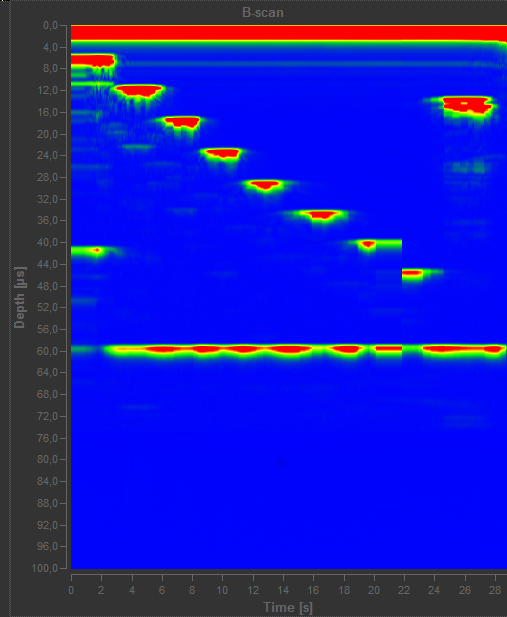
\includegraphics[height=13cm]{Daten/B-Scan1.png}
  \caption{Zweidimensionales Schnittbild vom ersten B-Scan.}
  \label{fig:BScan1}
\end{figure}

\begin{figure}
  \centering
  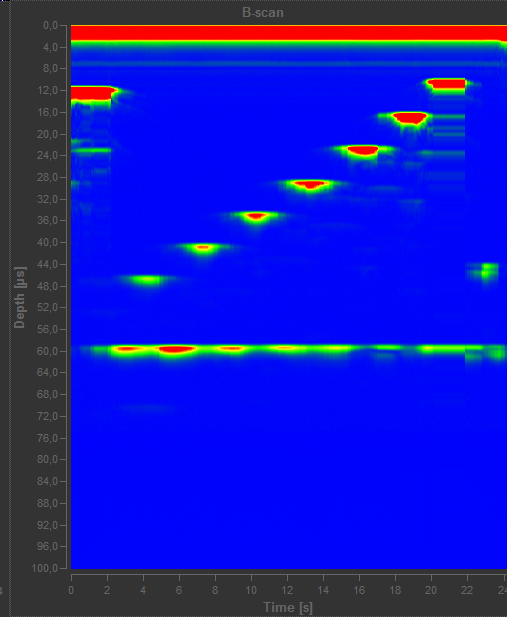
\includegraphics[height=13cm]{Daten/B-Scan2.png}
  \caption{Zweidimensionales Schnittbild vom zweiten B-Scan.}
  \label{fig:BScan2}
\end{figure}

\begin{figure}
  \centering
  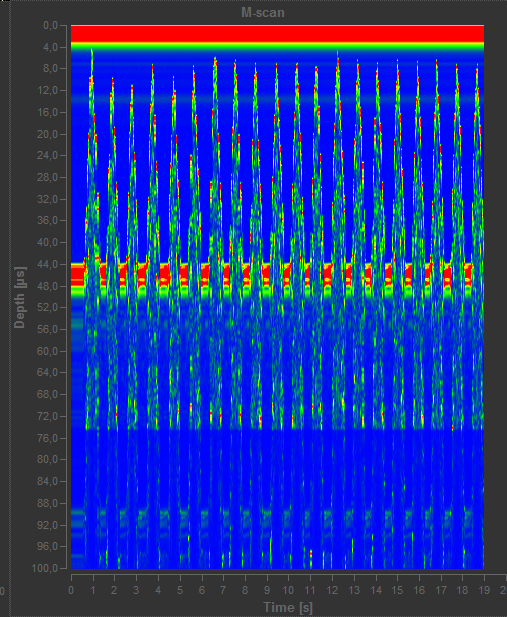
\includegraphics[height=13cm]{Daten/TM-Scan.png}
  \caption{TM-Scan.}
  \label{fig:TMScan}
\end{figure}

\begin{table}[h]
  \centering
  \begin{tabular}{S S S}
    \toprule
    {Störstelle} & {$s_\text{lit}/\si{\centi\meter}$} & {$d_\text{lit}
    /\si{\centi\meter}$}\\
    \midrule
    \text{c1} & 6.020 & 0.180 \\
    \text{c2} & 6.200 & 0.180 \\
    \text{a1} & 1.610 & 0.600 \\
    \text{a2} & 2.400 & 0.500 \\
    \text{a3} & 3.170 & 0.425 \\
    \text{a4} & 4.030 & 0.325 \\
    \text{a5} & 4.780 & 0.330 \\
    \text{a6} & 5.600 & 0.325 \\
    \text{a7} & 6.400 & 0.320 \\
    \text{a8} & 7.185 & 0.320 \\
    \text{b} & 1.980 & 1.030 \\
    \bottomrule
  \end{tabular}
  \caption{Messwerte für die Abstände $s_\text{lit}$ zwischen der unteren
  Kante und dem Mittelpunkt des jeweiligen Lochs und Durchmesser $d_\text{lit}$
  der Löcher am Acrylblock.}
  \label{tab:AbmessungenAcryl}
\end{table}

\begin{table}[h]
  \centering
  \begin{tabular}{S S S}
    \toprule
    {Störstelle} & {$t_\text{A,1}/\si{\micro\second}$} & {$t_\text{A,2}
    /\si{\micro\second}$}\\
    \midrule
    \text{c1} & 15.0 & 44.3 \\
    \text{c1} & 13.7 & 45.4 \\
    \text{a1} & 45.4 & 10.4 \\
    \text{a2} & 40.0 & 16.5 \\
    \text{a3} & 34.6 & 22.7 \\
    \text{a4} & 29.1 & 29.1 \\
    \text{a5} & 23.2 & 34.9 \\
    \text{a6} & 17.4 & 40.8 \\
    \text{a7} & 11.5 & 46.6 \\
    \text{a8} & 6.5 & \text{ } \\
    \text{b} & 41.3 & 11.7 \\
    \bottomrule
  \end{tabular}
  \caption{Messwerte für die Laufzeiten $t_\text{A,1}$ von der oberen Seite und
  $t_\text{A,2}$ von der unteren Seite bis zur jeweiligen Störstelle und zurück
  zum Sender.}
  \label{tab:AScanZeiten}
\end{table}

\begin{table}[h]
  \centering
  \begin{tabular}{S S S}
    \toprule
    {Störstelle} & {$s_\text{A,1}/\si{\centi\meter}$} & {$s_\text{A,2}
    /\si{\centi\meter}$}\\
    \midrule
    \text{c1} & 1.979 & 5.979 \\
    \text{c1} & 1.802 & 6.129 \\
    \text{a1} & 6.129 & 1.351 \\
    \text{a2} & 5.392 & 2.184 \\
    \text{a3} & 4.655 & 3.030 \\
    \text{a4} & 3.904 & 3.904 \\
    \text{a5} & 3.099 & 4.696 \\
    \text{a6} & 2.307 & 5.501 \\
    \text{a7} & 1.502 & 6.292 \\
    \text{a8} & 0.819 & \text{ } \\
    \text{b} & 5.569 & 1.529 \\
    \bottomrule
  \end{tabular}
  \caption{Berechnete Werte für die Strecken $s_\text{A,1}$ von der oberen Seite
  und $s_\text{A,2}$ von der unteren Seite bis zur jeweiligen Störstelle.}
  \label{tab:AScanStrecken}
\end{table}

\begin{table}[h]
  \centering
  \begin{tabular}{S S}
    \toprule
    {Störstelle} & {$d_\text{A}/\si{\centi\meter}$} \\
    \midrule
    \text{c1} & 0.082 \\
    \text{c1} & 0.109 \\
    \text{a1} & 0.560 \\
    \text{a2} & 0.464 \\
    \text{a3} & 0.355 \\
    \text{a4} & 0.232 \\
    \text{a5} & 0.246 \\
    \text{a6} & 0.232 \\
    \text{a7} & 0.246 \\
    \text{a8} & \text{ } \\
    \text{b} & 0.942 \\
    \bottomrule
  \end{tabular}
  \caption{Berechnete Werte für die Abmessungen $d_\text{A}$ der Störstellen.}
  \label{tab:AScanDicken}
\end{table}

\begin{table}[h]
  \centering
  \begin{tabular}{S S S S S S}
    \toprule
    {Störstelle} & {$t_\text{B,1}/\si{\micro\second}$} & {$t_\text{B,2}/
    \si{\micro\second}$} & {$s_\text{B,1}/\si{\centi\meter}$} & {$s_\text{B,2}/
    \si{\centi\meter}$} & {$d_\text{B}/\si{\centi\meter}$} \\
    \midrule
    \text{c1} & 13 & 43 & 1.365 & 5.460 & 1.215 \\
    \text{c2} & 13 & 44 & 1.365 & 5.597 & 1.079 \\
    \text{a1} & 45 & 10 & 5.733 & 0.956 & 1.352 \\
    \text{a2} & 40 & 17 & 5.051 & 1.911 & 1.079 \\
    \text{a3} & 34 & 22 & 4.232 & 2.594 & 1.215 \\
    \text{a4} & 29 & 29 & 3.549 & 3.549 & 0.942 \\
    \text{a5} & 23 & 34 & 2.730 & 4.232 & 1.079 \\
    \text{a6} & 17 & 40 & 1.911 & 5.051 & 1.079 \\
    \text{a7} & 11 & 46 & 1.092 & 5.870 & 1.079 \\
    \text{a8} & 05 & \text{ } & 0.273 & \text{ } & 8.177 \\
    \text{b} & 41 & 11 & 5.187 & 1.092 & 1.761 \\
    \bottomrule
  \end{tabular}
  \caption{Messwerte für die Laufzeiten $t_\text{B,1}$ und $t_\text{B,2}$ und
  die Strecken $s_\text{B,1}$ und $s_\text{B,2}$ zu den jeweiligen
  Störstellen, abgelesen aus den Abbildungen \ref{fig:BScan1} und
  \ref{fig:BScan2}, und die daraus berechneten Durchmessern $d_\text{B}$
  der jeweiligen
  Löcher.}
  \label{tab:BScanZeitenStreckenDicken}
\end{table}
